\documentclass[a4paper,11pt]{report}
\usepackage[T1]{fontenc}
\usepackage[utf8]{inputenc}
\usepackage[polish]{babel}
\usepackage{lmodern}
\usepackage{graphicx}
\usepackage{geometry}

\title{Implementacja algorytmu wyszukującego najkrótszą ścieżkę w grafie - A*. Porównanie z DFS oraz BFS.}
\author{Monika Litwin 200586}
\begin{document}
\maketitle

\begin{figure}
  \begin{center}
  \textbf{Algorytm A* }
\\
\begin{flushleft}

Jest to algorytm znajdowania najkrótszej ścieżki w grafie , w którym krawędzie posiadają wagi. Z dowolnego wierzchołka do wierzchołka przeznaczenia. Z dostępnych krawędzi, prowadzących do celu wybierana jest ta, o najmniejszej wadze. Sprawdzane jest też, czy obrana trasa jest poprawna (pomimo tego, że początkowa waga była najmiejsza, kolejne mogą być już dużo dłuższe od alternatywnych). Wówczas algorytm wybiera inną trasę. Tym sposobem A* znajduje zawsze najkrótszą drogę. Dzieje się to szybciej niż w przypadku innych podobnych algorytmów, np. Branch \& Bound, dzięki wykorzystaniu heurystyki. Jest to funkcja wyliczająca spodziewaną najkrótszą odległość między zadanymi wierzchołkami.

\end{flushleft}
  \end{center}
\end{figure}

\begin{figure}
  \begin{center}
  \textbf{Wyniki testów programu}
\\
\begin{flushleft}

W programie wywoływane były kolejno algorytmy wyszukujące - A*, BFS i DFS z tymi samymi parametrami (początkiem i celem). Mierzony był czas ich wykonania - do odnalezienia zadanego wierzchołka. Działo się tak dla grafów o różnej wielkości. Od 50 do 2.500.000 elementów. Poniżej zamieszczam wykres oraz wyniki pomiarów.
\begin{center} 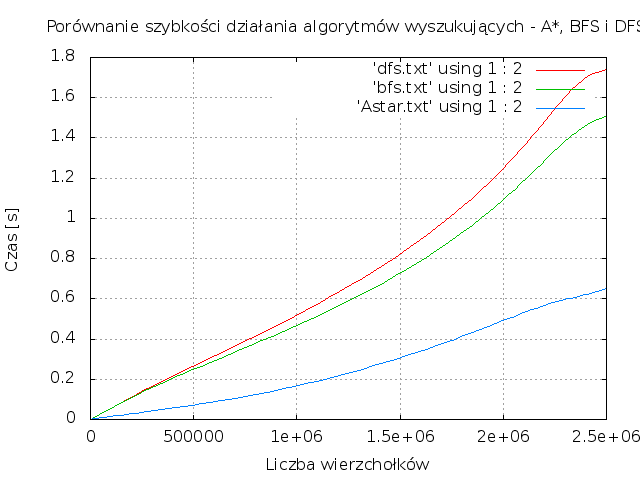
\includegraphics[scale=0.5]{./graf_przeszukiwanie.png}\end{center}
\end{flushleft}
  \end{center}
\end{figure}

\begin{figure}
  \begin{center}

  \begin{tabular}{|c|c|c|c|}
  \hline 
  Ilość wierzchołków & Czas - A* & Czas - BFS & Czas - DFS\\
  \hline
  50 & 0.00005 & 0.00002 & 0.00002\\
  \hline
  100 & 0.00034 & 0.00004 & 0.00003\\
  \hline
  1.000	& 0.0016 & 0.0002 & 0.0002\\
  \hline
  5.000	& 0.0021 & 0.0007 &  0.0003\\
  \hline
  10.000 & 0.003 & 0.001 & 0.001\\
  \hline
  50.000 & 0.001 & 0.002 & 0.002\\
  \hline
  100.000 & 0.04 &  0.05 & 0.08 \\
  \hline
  500.000 & 0.08 & 0.56  &  0.42\\
  \hline
  1.000.000 & 0.04 & 0.3 & 0.49 \\
  \hline
  1.500.000 &	0.2  & 0.35  & 0.42\\
  \hline
  2.000.000 & 0.4 & 1.11  &  1.14\\
  \hline
  2.100.000 & 0.7 & 1.12  &  1.37\\
  \hline
  2.200.000 & 0.52 & 1.32  & 1.44 \\
  \hline
  2.300.000 & 0.6 & 1.42  & 1.69 \\
  \hline
  2.400.000 & 0.62 & 1.47  & 1.72 \\
  \hline
  2.500.000 & 0.65 &  1.51 & 1.74 \\
  \hline
\end{tabular}
\end{center}
\end{figure}

\begin{figure}
  \begin{center}
\begin{flushleft}

Analizując wyniki pomiarów możemy zobaczyć, że dla mniejszych grafów lepsze czasy mają algorytmy DFS i BFS. Dla grafów liczących 50.000 wierzchołków i więcej ta tendencja się zmienia. Przy największych grafach - ponad 1.000.000 wierzchołków, A* jest zauważalnie bardziej wydajny, znacznie mniej wydajny jest BFS, a najmniej DFS.

\end{flushleft}
  \end{center}
\end{figure}

\begin{figure}
  \begin{center}
  \textbf{Wnioski}
\\
\begin{flushleft}

Wyniki analizy są zgodne z oczekiwaniami. Dla mniejszych grafów wydajniejsze są mniej skomplikowane algorytmy DFS i BFS. Przy większych grafach widoczna jest już przewaga algorytmu A*, który dzięki swoim dodatkowym funkcjom jest w stanie odrzucić ścieżki, które prawdopodobnie będą mało wydajne. BFS i DFS nie przeprowadzają takich szacować, tylko przeszukują w określonej kolejności wszystkie wierzchołki, aż do napotkania zadanego.

\end{flushleft}
  \end{center}
\end{figure}

\end{document}
